\part{Outils graphiques}

\section{Préambule}

\begin{cautionblock}
Les commandes \textit{graphiques} fournies par \ctex{ProfLycee} ont servi de base au package \ctex{tkz-grapheur} (\textsf{\href{https://ctan.org/pkg/tkz-grapheur}{[lien]}}) qui en reprend les éléments constructeurs.

Cette partie (hormis par exemple la section \textit{intervalles}) n'est plus officiellement \textit{maintenue}, mais elle reste présente dans le package et la documentation pour des raisons de rétro-compatibilité.
\end{cautionblock}

\section{Intervalles}\label{intervalles}

\subsection{Idée}

\begin{tipblock}
\cmaj{3.00a} L'idée est de proposer un environnement pour travailler sur des intervalles :

\begin{itemize}
	\item création de l'environnement (basé sur \TikZ) avec paramètres globaux (l'unité est le cm);
	\item commande pour créer un intervalle.
\end{itemize}
\vspace*{-\baselineskip}\leavevmode
\end{tipblock}

\begin{PresCodeTexPL}{listing only}
\begin{RepIntervalles}[clés]<options tikz>
	\tkzIntervalle[clés]{xmin}[labelxmin]{xmax}[labelxmax]
\end{RepIntervalles}
\end{PresCodeTexPL}

\begin{PresCodePL}{}
\begin{RepIntervalles}
	\tkzIntervalle{-4}{5}
\end{RepIntervalles}
\end{PresCodePL}

\subsection{Création de l'environnement}

\begin{PresCodeTexPL}{listing only}
\begin{RepIntervalles}[clés]<options tikz>
	%corps
\end{RepIntervalles}
\end{PresCodeTexPL}

\begin{cautionblock}
Les \Cle{clés} (globales pour l'ensemble de l'environnement, y compris pour la création des intervalles) disponibles pour l'environnement \ctex{RepIntervalles} sont :

\begin{itemize}
	\item \Cle{xmin} : valeur minimale pour l'axe ; \hfill{}défaut \Cle{-8}
	\item \Cle{xmax} : valeur maximale pour l'axe ; \hfill{}défaut \Cle{8}
	\item \Cle{Elargir} : coefficient d'alargisement de l'axe, en pourcentage de largeur; \hfill{}défaut \Cle{0.05}
	\item \Cle{Largeur} : largeur (en cm) de l'axe (hors élargissement) ; \hfill{}défaut \Cle{12}
	\item \Cle{Unite} : permet au code de calculer lui-même l'unité, sinon à donner en cm ; \hfill{}défaut \Cle{auto}
	\item \Cle{EpTrait} : épaisseur de base des tracés ; \hfill{}défaut \Cle{0.8pt}
	\item \Cle{Graduations} : liste des graduations (traits) à afficher ;
	\item \Cle{GraduationsAlt} : liste des graduations (traits un peu plus grands) à afficher ;
	\item \Cle{HautGrad} : hauteur de base des graduations ; \hfill{}défaut \Cle{7pt}
	\item \Cle{Hauteur} : hauteur des crochets des intervalles ; \hfill{}défaut \Cle{16pt}
	\item \Cle{Valeurs} : valeurs (formatées par \ctex{siunitx} !) à afficher sous l'axe ;
	\item \Cle{Police} : police globale des labels.\hfill{}défaut \Cle{\textbackslash normalsize\textbackslash normalfont}
\end{itemize}

L'argument optionnel, et entre \ctex{<...>}, permet de passer des options spécifiques à l'environnement \TikZ.
\end{cautionblock}

\begin{PresCodePL}{}
\begin{RepIntervalles}[Unite=1,xmin=-2,xmax=8,Graduations={-2,-1,...,8},GraduationsAlt={0,5}]
	%corps
\end{RepIntervalles}
\end{PresCodePL}

\begin{PresCodePL}{}
\begin{RepIntervalles}[Elargir=0.025,xmin=-100,xmax=200,Unite=auto,Largeur=10, Graduations={-100,-90,...,200},GraduationsAlt={-100,-50,...,200}, Valeurs={-100,-50,...,200},Police=\scriptsize]
	%corps
\end{RepIntervalles}
\end{PresCodePL}

\subsection{Représentation d'intervalles}

\begin{tipblock}
L'idée est de pouvoir représenter des intervalles dans l'environnement créé précédemment :

\begin{itemize}
	\item en prenant en compte le type d'intervalles et les bornes infinies ;
	\item en personnalisation la décoration éventuelle.
\end{itemize}
\vspace*{-\baselineskip}\leavevmode
\end{tipblock}

\begin{PresCodeTexPL}{listing only}
\begin{RepIntervalles}[clés]<options tikz>
	\tkzIntervalle[clés]{xmin}[labelxmin]{xmax}[labelxmax]
\end{RepIntervalles}
\end{PresCodeTexPL}

\begin{cautionblock}
Les \Cle{clés} (certains paramètres sont hérités des clés de l'environnement) disponibles pour la commande \ctex{\textbackslash tkzIntervalle} sont :

\begin{itemize}
	\item \Cle{Couleur} : couleur de base des tracés ; \hfill{}défaut \Cle{red}
	\item \Cle{Type} (parmi \ctex{FF / FO / OO / OF}) : choix du type d'intervalle ; \hfill{}défaut \Cle{FF}
	\item \Cle{NiveauV} : pour positionner l'intervalle décalé verticalement (en pourcentage de la hauteur) ; \hfill{}défaut \Cle{0}
	\item \Cle{Offset} : pour décaler légèrement la décoration (si superposition par exemple) ; \hfill{}défaut \Cle{0pt}
	\item \Cle{Decor} parmi \ctex{fond / zizgag / hach} : pour décorer l'intervalle (\ctex{hach/angle} pour choisir un angle des hachures) ; \hfill{}défaut \Cle{\{\}}
	\item \Cle{AffValeurs} : booléen pour afficher les valeurs de bornes ; \hfill{}défaut \Cle{false}
	\item \Cle{NumInf} : booléen pour afficher la borne inf grâce à \ctex{siunitx} ; \hfill{}défaut \Cle{true}
	\item \Cle{NumSup} : booléen pour afficher la borne sup grâce à \ctex{siunitx} ; \hfill{}défaut \Cle{true}
	\item \Cle{PosValeurs} : choix de la position des valeurs des bornes.\hfill{}défaut \Cle{above}
\end{itemize}

Les deux arguments obligatoires, et entre \ctex{\{...\}}, permettent de préciser les bornes de l'intervalle (en langage \TikZ, et avec \ctex{*} pour l'infini.)

\cmaj{3.00b} Les deux arguments optionnels correspondants, et entre \ctex{[...]}, permettent de spécifier les labels des bornes (dans le cas de valeurs rationnelles, ou bien dans le cas de valeurs littérales), et dans ce cas il sera opportun de mettre les booléens \Cle{NumInf/NumSup} à \Cle{false}.
\end{cautionblock}

\begin{PresCodePL}{}
\begin{RepIntervalles}[Elargir=0.025,xmin=-100,xmax=200,Unite=auto,Largeur=10, Graduations={-100,-90,...,200},GraduationsAlt={-100,-50,...,200}, Valeurs={-100,-50,...,200},Police=\scriptsize,EpTrait=0.6pt]
	\tkzIntervalle[AffValeurs]{-15}{175}
	\tkzIntervalle[Decor=fond,Couleur=teal,AffValeurs]{-56}{25}
	\tkzIntervalle[Decor=zigzag,NiveauV=1.5,Couleur=purple,AffValeurs,Type=OO]{0}{79}
\end{RepIntervalles}
\end{PresCodePL}

\begin{PresCodePL}{}
\begin{RepIntervalles}[Graduations={-8,-7,...,8}]
	\tkzIntervalle[Decor=fond,Offset=-1pt,AffValeurs,PosValeurs=below]{-2}{5}
	\tkzIntervalle[Type=OO,Couleur=blue,Decor=zigzag,Offset=1pt, AffValeurs,PosValeurs=below]{-7}{-1}
	\tkzIntervalle[Type=FO,Couleur=orange,NiveauV=1.25,Decor=hach,AffValeurs]{*}{6}
\end{RepIntervalles}
\end{PresCodePL}

\begin{PresCodePL}{}
%la commande \PlaceValeursAxe permet de placer des valeurs quelconques

\begin{RepIntervalles}[Graduations={-8,-7,...,8}]
	\PlaceValeursAxe{-10/3§$-\frac{10}{3}$,sqrt(13)§$\sqrt{13}$}
	\tkzIntervalle[Decor=fond,Offset=-1pt,AffValeurs,PosValeurs=below, NumInf=false,NumSup=false]{-2}[$a$]{5}[$b$]
	\tkzIntervalle[Couleur=blue,Type=OO,Decor=fond,Offset=1pt,AffValeurs, NumInf=false,NumSup=false]{-sqrt(5)}[$-\sqrt{5}$]{2/3}[$\tfrac23$]
\end{RepIntervalles}
\end{PresCodePL}

\pagebreak

\section{Repérage et tracé de courbes}\label{reperagetikz}

\subsection{Idée}

\begin{tipblock}
\cmaj{2.1.1} L'idée est de proposer des commandes \textit{simplifiées} pour tracer un repère, en \TikZ, avec :

\begin{itemize}
	\item axes et graduations, grille ;
	\item courbe.
\end{itemize}
\vspace*{-\baselineskip}\leavevmode
\end{tipblock}

\begin{noteblock}
Au niveau du code, il y aura donc plusieurs \textit{aspects} :

\begin{itemize}
	\item le paramétrage de la fenêtre graphique directement dans la déclaration de l'environnement ;
	\item les commandes de tracés avec options et clés.
\end{itemize}
\vspace*{-\baselineskip}\leavevmode
\end{noteblock}

\begin{PresCodeTexPL}{listing only}
%version basique
\begin{tikzpicture}[paramètres]
	%grille et axes
	\GrilleTikz[options][options grille ppale][options grille second.]
	\AxesTikz[options]
	\AxexTikz[options]{valeurs}
	\AxeyTikz[options]{valeurs}
	%courbe
	\CourbeTikz[options]{fonction}{valxmin:valxmax}
\end{tikzpicture}
\end{PresCodeTexPL}

\begin{PresCodeTexPL}{listing only}
%version simplifiée
\begin{tikzpicture}[<paramètres>]
	%grille et axes
	\FenetreSimpleTikz[opt](opt axes)<opt axe Ox>{liste valx}<opt axe Oy>{liste valy}
	%courbe
	\CourbeTikz[options]{fonction}{valxmin:valxmax}
\end{tikzpicture}
\end{PresCodeTexPL}

\begin{PresCodeSortiePL}{text only}
\begin{tikzpicture}%
	[x=0.1cm,y=0.0167cm, %unités
	xmin=0,xmax=60,xgrille=5,xgrilles=5, %axe Ox
	ymin=0,ymax=240,ygrille=30,ygrilles=30] %axe Oy
	\FenetreSimpleTikz<Police=\small>{0,5,...,55}<Police=\small>{0,30,...,210} %repère
	\CourbeTikz[line width=1.25pt,CouleurVertForet,samples=250]%
		{\x*\x*exp(-0.05*\x)+1}{0:60} %courbe
\end{tikzpicture}
\end{PresCodeSortiePL}

\subsection{Commandes, clés et options}

\begin{noteblock}
Les \Cle{paramètres} nécessaires à la bonne utilisation des commandes suivantes sont à déclarer directement dans l'environnement \ctex{tikzpicture}, seules les versions \og x \fg{}  sont présentées ici:

\begin{itemize}
	\item \Cle{xmin}, stockée dans \ctex{\textbackslash{}xmin} ;\hfill{}défaut \Cle{-3}
	\item \Cle{xmax}, stockée dans \ctex{\textbackslash{}xmax} ;\hfill{}défaut \Cle{3}
	\item \Cle{Ox}, stockée dans \ctex{\textbackslash{}axexOx}, origine de l'axe $(Ox)$ ;\hfill{}défaut \Cle{0}
	\item \Cle{xgrille}, stockée dans \ctex{\textbackslash{}xgrille}, graduation principale ;\hfill{}défaut \Cle{1}
	\item \Cle{xgrilles}, stockée dans \ctex{\textbackslash{}xgrilles}, graduation secondaire.\hfill{}défaut \Cle{0.5}
\end{itemize}

La fenêtre d'affichage (de sortie) sera donc \textit{portée} par le rectangle de coins $(\text{xmin};\text{ymin})$ et $(\text{xmax};\text{ymax})$ ; ce qui correspond en fait à la fenêtre \TikZ{} \textit{portée} par le rectangle de coins $(\text{xmin-Ox};\text{ymin-Oy})$ et $(\text{xmax-Ox};\text{ymax-Oy})$.

\smallskip

Les commandes ont -- pour certaines -- pas mal de \Cle{clés} pour des réglages fins, mais dans la majorité des cas elles ne sont pas forcément \textit{utiles}.
\end{noteblock}

\begin{PresCodeTexPL}{listing only}
%...code tikz
	\GrilleTikz[options][options grille ppale][options grille second.]
\end{PresCodeTexPL}

\begin{cautionblock}
Cette commande permet de tracer une grille principale et/ou une grille secondaire :

\begin{itemize}
	\item les premières \Cle{clés} sont les booléens \Cle{Affp} et \Cle{Affs} qui affichent ou non les grilles ;

	\hfill~défaut \Cle{true}
	\item les options des grilles sont en \TikZ. \hfill~défaut \Cle{thin,lightgray} et \Cle{very thin,lightgray}
\end{itemize}
\vspace*{-\baselineskip}\leavevmode
\end{cautionblock}

\begin{PresCodeTexPL}{listing only}
\begin{tikzpicture}%
	[x=0.1cm,y=0.0167cm, %unités
	xmin=0,xmax=60,xgrille=5,xgrilles=5, %axe Ox
	ymin=0,ymax=240,ygrille=30,ygrilles=30] %axe Oy
	\GrilleTikz
\end{tikzpicture}
~~
\begin{tikzpicture}%
	[x=0.1cm,y=0.0167cm, %unités
	xmin=0,xmax=60,xgrille=5,xgrilles=5, %axe Ox
	ymin=0,ymax=240,ygrille=30,ygrilles=30] %axe Oy
	\GrilleTikz[Affp=false][][orange,densely dotted]
\end{tikzpicture}
\end{PresCodeTexPL}

\begin{PresCodeSortiePL}{text only}
\hfill~
\begin{tikzpicture}%
	[x=0.1cm,y=0.0167cm, %unités
	xmin=0,xmax=60,xgrille=5,xgrilles=5, %axe Ox
	ymin=0,ymax=240,ygrille=30,ygrilles=30] %axe Oy
	\GrilleTikz
\end{tikzpicture}
~~
\begin{tikzpicture}%
	[x=0.1cm,y=0.0167cm, %unités
	xmin=0,xmax=60,xgrille=5,xgrilles=5, %axe Ox
	ymin=0,ymax=240,ygrille=30,ygrilles=30] %axe Oy
	\GrilleTikz[Affp=false][][orange,densely dotted]
\end{tikzpicture}
\hfill~
\end{PresCodeSortiePL}

\pagebreak

\begin{PresCodeTexPL}{listing only}
%...code tikz
	\AxesTikz[options]
\end{PresCodeTexPL}

\begin{cautionblock}
Cette commande permet de tracer les axes, avec des \Cle{clés} :

\begin{itemize}
	\item \Cle{Epaisseur} qui est l'épaisseur des axes ; \hfill~défaut \Cle{1pt}
	\item \Cle{Police} qui est le style des labels des axes  ; \hfill~défaut \Cle{\textbackslash{}normalsize\textbackslash{}normalfont}
	\item \cmaj{2.1.2} \Cle{ElargirOx} qui est le \% l'élargissement \Cle{global} ou \Cle{G/D} de l'axe $(Ox)$ ;
	
	\hfill~défaut \Cle{0/0.05}
	\item \cmaj{2.1.2} \Cle{ElargirOy} qui est le \% l'élargissement \Cle{global} ou \Cle{B/H} de l'axe $(Oy)$ ;
	
	\hfill~défaut \Cle{0/0.05}
	\item \Cle{Labelx} qui est le label de l'axe $(Ox)$ ; \hfill~défaut \Cle{\${}x\$}
	\item \Cle{Labely} qui est le label de l'axe $(Oy)$ ; \hfill~défaut \Cle{\${}y\$}
	\item \Cle{AffLabel} qui est le code pour préciser quels labels afficher, entre \Cle{x}, \Cle{y} ou \Cle{xy} ;
	
	\hfill~défaut \Cle{vide}
	\item \Cle{PosLabelx} pour la position du label de $(Ox)$ en bout d'axe ; \hfill~défaut \Cle{right}
	\item \Cle{PosLabely} pour la position du label de $(Oy)$ en bout d'axe ; \hfill~défaut \Cle{above}
	\item \Cle{EchelleFleche} qui est l'échelle de la flèche des axes ; \hfill~défaut \Cle{1}
	\item \Cle{TypeFleche} qui est le type de la flèche des axes.\hfill~défaut \Cle{latex}
\end{itemize}
\vspace*{-\baselineskip}\leavevmode
\end{cautionblock}

\begin{PresCodeTexPL}{listing only}
%code tikz
\AxesTikz

%code tikz
\AxesTikz%
	[AffLabel=xy,Labelx={Nombre de jours},Labely={Nombre d'individus infectés, en centaines},%
	PosLabelx={above left},PosLabely={above right},%
	Police=\small\sffamily,ElargirOx=0,ElargirOy=0]
\end{PresCodeTexPL}

\begin{PresCodeSortiePL}{text only}
\hfill~
\begin{tikzpicture}%
	[x=0.1cm,y=0.0167cm, %unités
	xmin=0,xmax=60,xgrille=5,xgrilles=5, %axe Ox
	ymin=0,ymax=240,ygrille=30,ygrilles=30] %axe Oy
	\AxesTikz
\end{tikzpicture}
~~
\begin{tikzpicture}%
	[x=0.1cm,y=0.0167cm, %unités
	xmin=0,xmax=60,xgrille=5,xgrilles=5, %axe Ox
	ymin=0,ymax=240,ygrille=30,ygrilles=30] %axe Oy
	\AxesTikz%
	[AffLabel=xy,Labelx={Nombre de jours},
	Labely={Nombre d'individus infectés, en centaines},%
	PosLabelx={above left},PosLabely={above right},%
	ElargirOx=0,ElargirOy=0,
	Police=\small\sffamily]
\end{tikzpicture}
\hfill~
\end{PresCodeSortiePL}

\pagebreak

\begin{PresCodeTexPL}{listing only}
%...code tikz
	\AxexTikz[options]{valeurs}
	\AxeyTikz[options]{valeurs}
	%ou
	\AxexyTikz[optionsOx][optionsOy]{valeursOx}{valeursOy}
\end{PresCodeTexPL}

\begin{cautionblock}
Ces commande permet de tracer les graduations des axes, avec des \Cle{clés} identiques pour les deux directions :

\begin{itemize}
	\item \Cle{Epaisseur} qui est l'épaisseur des graduations ; \hfill~défaut \Cle{1pt}
	\item \Cle{Police} qui est le style des labels des graduations ; \hfill~défaut \Cle{\textbackslash{}normalsize\textbackslash{}normalfont}
	\item \Cle{PosGrad} qui est la position des graduations par rapport à l'axe ; \hfill~défaut \Cle{below} et \Cle{left}
	\item \Cle{HautGrad} qui est la hauteur des graduations (sous la forme \Cle{lgt} ou \Cle{lgta/lgtb}) ;
	
	\hfill~défaut \Cle{4pt}
	\item le booléen \Cle{AffGrad} pour afficher les valeurs (formatés avec \ctex{num} donc dépendant de \ctex{sisetup}) des graduations  ; \hfill~défaut \Cle{true}
	\item le booléen \Cle{AffOrigine} pour afficher la graduation de l'origine ; \hfill~défaut \Cle{true}
	\item le booléen \Cle{Annee} qui permet de ne pas formater les valeurs des graduations (type \textsf{année}) ;
	
	\hfill~défaut \Cle{false}
	\item \cmaj{2.5.6} le booléen \Cle{Trigo} (uniquement pour l'axe $(Ox)$) pour des graduations libres en radians ;
	
	\hfill~défaut \Cle{false}
	\item \cmaj{2.5.6} le booléen \Cle{Dfrac} (uniquement pour l'axe $(Ox)$ en \Cle{Trigo}) pour forcer les fractions en \textit{grand} ;
	
	\hfill~défaut \Cle{false}
	\item \cmaj{2.7.0} le booléen \Cle{Frac} (uniquement pour l'axe $(Oy)$) pour forcer les graduations en fraction (taille normale).
	
	\hfill~défaut \Cle{false}
\end{itemize}

\cmaj{3.04b} L'argument obligatoire permet de spécifier les valeurs des graduations (la valeur \ctex{auto} permet d'utiliser automatiquement les valeurs initiales du paramétrage de la fenêtre \ctex{xmin/xgrille/xmax} et/ou \ctex{ymin/ygrille/ymax}, donc les clés \Cle{ElargirOx/ElargirOy} sont intéressantes dans ce cas).

\end{cautionblock}

\begin{PresCodeTexPL}{listing only}
%code tikz
	\AxexTikz[Police=\small]{0,5,...,55}
	\AxeyTikz[Police=\small]{0,30,...,210}
%code tikz
	\AxexTikz[Police=\small,HautGrad=0pt/4pt]{0,5,...,55}
	\AxeyTikz[AffGrad=false,HautGrad=6pt]{0,30,...,210}
%des axes fictifs (en gris) sont rajoutés pour la lisibilité du code de sortie
\end{PresCodeTexPL}

\begin{PresCodeSortiePL}{text only}
\hfill~
\begin{tikzpicture}%
	[x=0.1cm,y=0.0167cm, %unités
	xmin=0,xmax=60,xgrille=5,xgrilles=5, %axe Ox
	ymin=0,ymax=240,ygrille=30,ygrilles=30] %axe Oy
	\draw[gray,line width=1.25pt,->,>=latex] ({\xmin-\axexOx},0) -- ({\xmax-\axexOx},0) ;
	\draw[gray,line width=1.25pt,->,>=latex] (0,{\ymin-\axeyOy}) -- (0,{\ymax-\axeyOy}) ;
	\AxexTikz[Police=\small]{0,5,...,55}
	\AxeyTikz[Police=\small]{0,30,...,210}
\end{tikzpicture}
~~
\begin{tikzpicture}%
	[x=0.1cm,y=0.0167cm, %unités
	xmin=0,xmax=60,xgrille=5,xgrilles=5, %axe Ox
	ymin=0,ymax=240,ygrille=30,ygrilles=30] %axe Oy
	\draw[gray,line width=1.25pt,->,>=latex] ({\xmin-\axexOx},0) -- ({\xmax-\axexOx},0) ;
	\draw[gray,line width=1.25pt,->,>=latex] (0,{\ymin-\axeyOy}) -- (0,{\ymax-\axeyOy}) ;
	\AxexTikz[Police=\small,HautGrad=0pt/4pt]{0,5,...,55}
	\AxeyTikz[AffGrad=false,HautGrad=6pt]{0,30,...,210}
\end{tikzpicture}
\hfill~
\end{PresCodeSortiePL}

\begin{PresCodeTexPL}{listing only}
\begin{tikzpicture}[x=2cm,y=1cm,xmin=0,xmax={2*pi},xgrille=0.5,xgrilles=0.25,
	ymin=-1.15,ymax=1.15,ygrille=0.5,ygrilles=0.25]
	\GrilleTikz \AxesTikz
	\AxexTikz[Trigo]{{pi/6},{pi/4},{pi/3},{pi/2},{2*pi/3},%
		{3*pi/4},{5*pi/6},pi,{7*pi/6},{5*pi/4}}
	\CourbeTikz[thick,blue,samples=250]{cos(deg(\x))}{0:2*pi}
\end{tikzpicture}
\end{PresCodeTexPL}

\begin{PresCodeSortiePL}{text only}
\begin{tikzpicture}
	[x=2cm,y=1cm,xmin=0,xmax={2*pi},xgrille=0.5,xgrilles=0.25,
	ymin=-1.15,ymax=1.15,ygrille=0.5,ygrilles=0.25]
	\GrilleTikz \AxesTikz
	\AxexTikz[Trigo]{{pi/6},{pi/4},{pi/3},{pi/2},{2*pi/3},%
		{3*pi/4},{5*pi/6},pi,{7*pi/6},{5*pi/4}}
	\CourbeTikz[thick,blue,samples=250]{cos(deg(\x))}{0:2*pi}
\end{tikzpicture}
\end{PresCodeSortiePL}

\begin{noteblock}
La clé \Cle{Trigo} utilise, en interne, une commande qui permet de \textit{transformer} les abscisses, données en langage \TikZ, en fraction en \LaTeX.
\end{noteblock}

\begin{PresCodePL}{}
$\AffAngleRadian{0}$ \quad $\AffAngleRadian{pi}$ \quad $\AffAngleRadian{pi/4}$ \quad 
$\AffAngleRadian{2*pi/3}$ \quad $\AffAngleRadian{-2*pi/3}$ \quad $\AffAngleRadian*{-2*pi/3}$
\end{PresCodePL}

\subsection{Commandes annexes}

\begin{noteblock}
Il existe, de manière marginale, quelques commandes complémentaires qui ne seront pas trop détaillées mais qui sont existent :

\begin{itemize}
	\item \ctex{FenetreTikz} qui restreint les tracés à la fenêtre (utile pour des courbes qui \textit{débordent}) ;
	\item \ctex{FenetreSimpleTikz} qui permet d'automatiser le tracé des grilles/axes/graduations dans leurs versions par défaut, avec peu de paramétrages ;
	\item \ctex{OrigineTikz} pour rajouter le libellé de l'origine si non affiché par les axes.
\end{itemize}
\vspace*{-\baselineskip}\leavevmode
\end{noteblock}

\begin{PresCodeTexPL}{listing only}
%code tikz
	\FenetreTikz                %on restreint les tracés
	\FenetreSimpleTikz%
		[options](opt axes)<opt axe Ox>{valeurs Ox}<opt axe Oy>{valeurs Oy}
\end{PresCodeTexPL}

\begin{tipblock}
L'idée est de proposer, en \textit{complément}, une commande simplifiée pour tracer une courbe en \TikZ.

\textbf{NB} : Il est également possible d'utiliser \ctex{xint} comme \textit{moteur} de tracé.
\end{tipblock}

\begin{PresCodeTexPL}{listing only}
%...code tikz
\CourbeTikz[options]{formule tikz}{domaine}
\end{PresCodeTexPL}

\begin{cautionblock}
Cette commande permet de rajouter une courbe sur le graphique (sans se soucier de la transformation de son expression) avec les arguments :

\begin{itemize}
	\item \Cle{optionnels} qui sont - en \TikZ{} - les paramètres du tracé ;
	\item le premier \textit{obligatoire}, est - en langage \TikZ{} - l'expression de la fonction à tracer, donc avec \ctex{\textbackslash{}x} comme variable ;
	\item le second \textit{obligatoire} est le domaine du tracé, sous la forme \ctex{valxmin:valxmax}.
\end{itemize}
\vspace*{-\baselineskip}\leavevmode
\end{cautionblock}

\begin{PresCodeTexPL}{listing only}
\begin{tikzpicture}[x=0.1cm,y=0.0167cm, %unités
	xmin=0,xmax=60,xgrille=5,xgrilles=5, %axe Ox
	ymin=0,ymax=240,ygrille=30,ygrilles=30] %axe Oy
	\FenetreSimpleTikz%
		<Police=\small>{auto}%
		<Police=\small>{auto} %repère
	\CourbeTikz[line width=1.25pt,CouleurVertForet,samples=250]%
		{\x*\x*exp(-0.05*\x)+1}{0:60} %courbe
\end{tikzpicture}
\end{PresCodeTexPL}

\begin{PresCodeSortiePL}{text only}
\begin{tikzpicture}%
	[x=0.1cm,y=0.0167cm, %unités
	xmin=0,xmax=60,xgrille=5,xgrilles=5,ymin=0,ymax=240,ygrille=30,ygrilles=30]
	\FenetreSimpleTikz%
		<Police=\small>{auto}<Police=\small>{0,30,...,240} %repère
	\CourbeTikz[line width=1.25pt,CouleurVertForet,samples=250]%
		{\x*\x*exp(-0.05*\x)+1}{0:60} %courbe
\end{tikzpicture}
\end{PresCodeSortiePL}

\subsection{Repère non centré en O}

\begin{tipblock}
Parfois on est amené à travailler dans des repères qui n'ont pas forcément pour origine $(0;0)$. De ce fait - pour éviter des erreurs de \ctex{dimension too large} liées à \TikZ{} - il faut \textit{décaler les axes} pour se ramener à une origine en $O$. L'idée est donc d'utiliser les commandes précédentes, sans se soucier des éventuelles transformations !
\end{tipblock}

\begin{PresCodePL}{}
\begin{tikzpicture}[x=0.35cm,y=0.07cm,Ox=1992,xmin=1992,xmax=2010,%
	xgrille=2,xgrilles=1,Oy=1640,ymin=1640,ymax=1710,ygrille=10,ygrilles=5]
	\FenetreSimpleTikz<Annee,Police=\scriptsize>{1992,1994,...,2008}{1640,1650,...,1700}
	\FenetreTikz
	\CourbeTikz[line width=1.25pt,orange,samples=500]{-(\x-2000)*(\x-2000)+1700}{\xmin:\xmax}
\end{tikzpicture}
\end{PresCodePL}

\subsection{Utilisation de xint pour des courbes}\label{courbexint}

\begin{tipblock}
Pour certaines fonctions, les capacités de calculs de \ctex{tikz} ne permettent pas de tracer la courbe (les fameuses erreurs \ctex{dimension too large}).

\ctex{ProfLycee} propose une commande pour tracer une courbe en utilisant les capacités de calculs de \ctex{xint}, qui est donc à insérer dans un environnement \ctex{tikzpicture}.
\end{tipblock}

\begin{PresCodeTexPL}{listing only}
%la fonction est à donner en langage xint (argument #2)
%le domaine est à donner sous la forme début..[pas]..fin (argument #3)
\CourbeTikzXint[options tikz]{fonction}{domaine}
\end{PresCodeTexPL}

\begin{PresCodePL}{}
On souhaite tracer la courbe de la fonction $f(x)=\dfrac{\num{94900}}{(x-130)^2-5}$ sur $\IntervalleFF{0}{100}$.

\begin{tikzpicture}[x=0.05cm,y=0.05cm,xmin=0,xmax=100,xgrille=10,%
	xgrilles=10,ymin=0,ymax=100,ygrille=10,ygrilles=10]
	\FenetreSimpleTikz
		<Police=\scriptsize>{0,10,...,100}
		<Police=\scriptsize>{0,10,...,100}
	\FenetreTikz
	\CourbeTikzXint[very thick,blue]{94900/(x-130)^2-5}{0..[0.5]..100}
\end{tikzpicture}
\end{PresCodePL}

\pagebreak

\section{L'outil \og SplineTikz \fg}

\subsection{Courbe d'interpolation}

\begin{noteblock}
On va utiliser les notions suivantes pour paramétrer le tracé \og automatique \fg{} grâce à  \ctex{..controls} :
%
\begin{itemize}
	\item il faut rentrer les \textcolor{purple}{\textsf{points de contrôle}} ;
	\item il faut préciser les \textcolor{CouleurVertForet}{\textsf{pentes des tangentes}} (pour le moment on travaille avec les mêmes à gauche et à droite\ldots) ;
	\item on peut \og affiner \fg{} les portions de courbe en paramétrant des \textcolor{BleuCadet}{\textsf{coefficients}} (voir un peu plus loin\ldots).
\end{itemize}

\medskip

Pour déclarer les paramètres :
%
\begin{itemize}
	\item liste des points de contrôle (minimum 2 !!) par : \verb|x1/y1/d1§x2/y2/d2§...| avec les points \pverb|(xi;yi)| et \vverb|f'(xi)=di| ;
	\item coefficients de contrôle par \verb|coeffs=...| :
	\begin{itemize}
		\item \averb|coeffs=x| pour mettre tous les coefficients à x ;
		\item \averb|coeffs=C1§C2§...| pour spécifier les coefficients par portion (donc il faut avoir autant de § que pour les points !) ;
		\item \averb|coeffs=C1G/C1D§...| pour spécifier les coefficients par portion et par partie gauche/droite ;
		\item on peut mixer avec \averb|coeffs=C1§C2G/C2D§...|.
	\end{itemize}
\end{itemize}
\vspace*{-\baselineskip}\leavevmode
\end{noteblock}

\subsection{Code, clés et options}

\begin{PresCodeTexPL}{listing only}
\begin{tikzpicture}
...
\SplineTikz[options]{liste}
...
\end{tikzpicture}
\end{PresCodeTexPL}

\begin{cautionblock}
Certains paramètres et \Cle{clés} peuvent être gérés directement dans la commande \ctex{\textbackslash SplineTikz} :
%
\begin{itemize}
	\item la couleur de la courbe par la {clé} \Cle{Couleur} ;\hfill{}défaut \Cle{red}
	\item l'épaisseur de la courbe par la {clé} \Cle{Epaisseur} ;\hfill{}défaut \Cle{1.25pt}
	\item du style supplémentaire pour la courbe peut être rajouté, grâce à la {clé} \Cle{Style} ;\hfill{}défaut \Cle{vide}
	\item les coefficients de \textit{compensation} gérés par la {clé} \Cle{Coeffs} ;\hfill{}défaut \Cle{3}
	\item les points de contrôle , affichés ou non par la {clé booléenne} \Cle{AffPoints} ;\hfill{}défaut \Cle{false}
	\item la taille des points de contrôle est géré par la {clé} \Cle{TaillePoints}.\hfill{}défaut \Cle{2pt}
\end{itemize}
\vspace*{-\baselineskip}\leavevmode
\end{cautionblock}

\subsection{Compléments sur les coefficients de \og compensation \fg}

\begin{tipblock}
Le choix a été fait ici, pour \textit{simplifier} le code, le travailler sur des courbes de Bézier.

Pour \textit{simplifier} la gestion des nombres dérivés, les points de contrôle sont gérés par leurs coordonnées \textit{polaires}, les \textsf{coefficients de compensation} servent donc -- grosso modo -- à gérer la position radiale.

\smallskip

Le coefficient \Cle{3} signifie que, pour une courbe de Bézier entre $x=a$ et $x=b$, les points de contrôles seront situés à une distance radiale de $\frac{b-a}{3}$.

Pour \textit{écarter} les points de contrôle, on peut du coup \textit{réduire} le coefficient de compensation !

\medskip

Pour des intervalles \textit{étroits}, la \textit{pente} peut paraître abrupte, et donc le(s) coefficient(s) peuvent être modifiés, de manière fine.

\medskip

Si jamais il existe (un ou) des points \textit{anguleux}, le plus simple est de créer les splines en plusieurs fois.
\end{tipblock}

\subsection{Exemples}

\begin{PresCodePL}{tikz lower}
%code tikz
\def\x{0.9cm}\def\y{0.9cm}
\def\xmin{-1}\def\xmax{11}\def\xgrille{1}\def\xgrilles{0.5}
\def\ymin{-1}\def\ymax{5}\def\ygrille{1}\def\ygrilles{0.5}
%axes et grilles
\draw[xstep=\xgrilles,ystep=\ygrilles,line width=0.6pt,lightgray!50] (\xmin,\ymin) grid (\xmax,\ymax);
\draw[line width=1.5pt,->,gray,>=latex] (\xmin,0)--(\xmax,0) ;
\draw[line width=1.5pt,->,gray,>=latex] (0,\ymin)--(0,\ymax) ;
\foreach \x in {0,1,...,10} {\draw[gray,line width=1.5pt] (\x,4pt) -- (\x,-4pt) ;}
\foreach \y in {0,1,...,4} {\draw[gray,line width=1.5pt] (4pt,\y) -- (-4pt,\y) ;}
\draw[darkgray] (1,-4pt) node[below,font=\sffamily] {1} ;
\draw[darkgray] (-4pt,1) node[left,font=\sffamily] {1} ;
%splines
\def\LISTE{0/1/0§4/3.667/-0.333§7.5/1.75/0§9/2/-0.333§10/0/-10}
\SplineTikz[AffPoints,Coeffs=3,Couleur=red]{\LISTE}
\end{PresCodePL}

\begin{noteblock}
Avec des explications utiles à la compréhension :

\begin{center}
\begin{tikzpicture}[x=0.9cm,y=0.9cm,xmin=-1,xmax=11,xgrille=1,xgrilles=0.5,ymin=-1,ymax=7,ygrille=1,ygrilles=0.5]
	\genfenetre
	\SplineTikz[AffPoints]{0/1/0§4/3.667/-0.333§7.5/1.75/0§9/2/-0.333§10/0/-10}
	\gennotice
	\gentangentes
	\listecoeffs{3}{3}{3}{3}
\end{tikzpicture}
\end{center}
\end{noteblock}

\subsection{Avec une gestion plus fine des \og coefficients \fg}

\begin{noteblock}
Dans la majorité des cas, le \textit{coefficient} \textcircled{3} permet d'obtenir une courbe (ou une portion) très satisfaisante !

Dans certains cas, il se peut que la portion paraisse un peu trop \og abrupte \fg{}.

On peut dans ce cas \textit{jouer} sur les coefficients de cette portion pour \textit{arrondir} un peu tout cela (\textit{ie} diminuer le \textsf{coeff}\ldots)!

\begin{center}
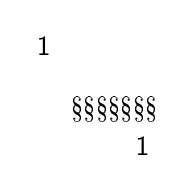
\begin{tikzpicture}[x=0.9cm,y=0.9cm,xmin=-1,xmax=11,xgrille=1,xgrilles=0.5,ymin=-1,ymax=7,ygrille=1,ygrilles=0.5]
	\genfenetre
	\draw (1,-4pt) node[below,font=\sffamily] {1} ;
	\draw (-4pt,1) node[left,font=\sffamily] {1} ;
	\def\LISTE{0/1/0§4/3.667/-0.333§7.5/1.75/0§9/2/-0.333§10/0/-10}
	\SplineTikz[AffPoints,Coeffs=3§3§3§2/1]{\LISTE}
	\gennotice
	\listecoeffs{3/3}{3/3}{3/3}{2/1}
	\end{tikzpicture}
\end{center}
\end{noteblock}

\begin{PresCodeTexPL}{listing only}
...
%splines
\def\LISTE{0/1/0§4/3.667/-0.333§7.5/1.75/0§9/2/-0.333§10/0/-10}
\SplineTikz[AffPoints,Coeffs=3§3§3§2/1]{\LISTE}
...
\end{PresCodeTexPL}

\begin{PresCodeSortiePL}{text only}
\begin{center}
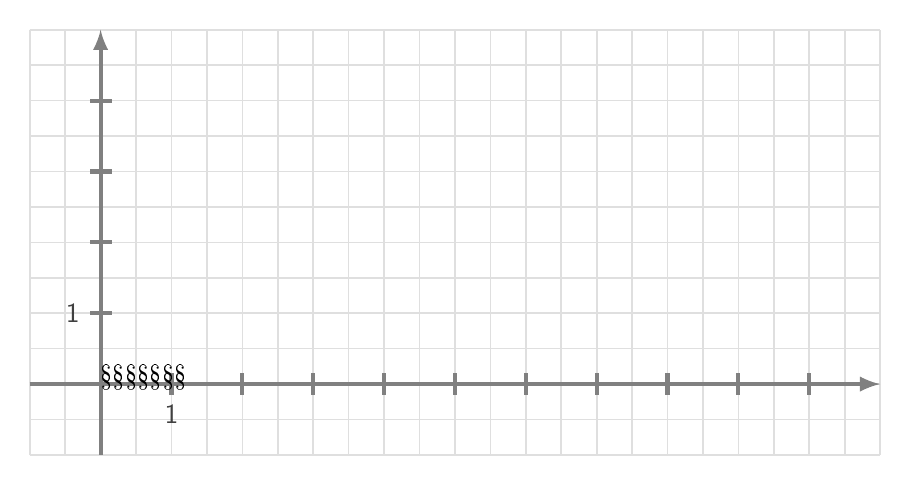
\begin{tikzpicture}[x=0.9cm,y=0.9cm,xmin=-1,xmax=11,xgrille=1,xgrilles=0.5,ymin=-1,ymax=5,ygrille=1,ygrilles=0.5]
	%axes et grilles
	\draw[xstep=\xgrilles,ystep=\ygrilles,line width=0.3pt,lightgray!50] (\xmin,\ymin) grid (\xmax,\ymax);
	\draw[xstep=\xgrilles,ystep=\ygrilles,line width=0.6pt,lightgray!50] (\xmin,\ymin) grid (\xmax,\ymax);
	\draw[line width=1.5pt,->,gray,>=latex] (\xmin,0)--(\xmax,0) ;
	\draw[line width=1.5pt,->,gray,>=latex] (0,\ymin)--(0,\ymax) ;
	\foreach \x in {0,1,...,10} {\draw[gray,line width=1.5pt] (\x,4pt) -- (\x,-4pt) ;}
	\foreach \y in {0,1,...,4} {\draw[gray,line width=1.5pt] (4pt,\y) -- (-4pt,\y) ;}
	\draw[darkgray] (1,-4pt) node[below,font=\sffamily] {1} ;
	\draw[darkgray] (-4pt,1) node[left,font=\sffamily] {1} ;
	\def\LISTE{0/1/0§4/3.667/-0.333§7.5/1.75/0§9/2/-0.333§10/0/-10}
	\SplineTikz[AffPoints,Coeffs=3§3§3§2/1]{\LISTE}
\end{tikzpicture}
\end{center}
\end{PresCodeSortiePL}

\subsection{Conclusion}

\begin{noteblock}
Le plus \og simple \fg{} est donc:
%
\begin{itemize}
	\item de déclarer la liste des points de contrôle, grâce à \ctex{\textbackslash def\textbackslash LISTE\{x1/y1/d1§x2/y2/d2§...\}} ;
	\item de saisir la commande \ctex{\textbackslash SplineTikz[...]\{\textbackslash LISTE\}} ;
	\item d'ajuster les options et coefficients en fonction du rendu !
\end{itemize}
\vspace*{-\baselineskip}\leavevmode
\end{noteblock}

\newpage

\section{Génération de la courbe d'interpolation}\label{gensplines}

\subsection{Intro}

\begin{tipblock}
\cmaj{3.01c} Dans le cas où la courbe d'interpolation est destinée à être (ré)utilisée, comme pour illustrer des intégrales par exemple, il est possible de \textit{générer} une macro pour le tracé, afin de faire la représentation ou l'exploitation \textit{à la main}.
\end{tipblock}

\begin{PresCodeTexPL}{listing only}
\begin{tikzpicture}
	...
	\GenereSplineTikz[options]{liste}[\nomdutracé]
	\draw[options] \nomdutracé ;
	...
\end{tikzpicture}
\end{PresCodeTexPL}

\begin{cautionblock}
Cela permet de générer le tracé de la courbe d'interpolation, avec le même format de données que pour la commande de \textit{tracé} :

\begin{itemize}
	\item la liste des points de contrôle (minimum 2 !!)  définie par : \verb|x1/y1/d1§x2/y2/d2§...| avec les points \pverb|(xi;yi)| et \vverb|f'(xi)=di| ;
	\item les coefficients de contrôle par \verb|coeffs=...| :
	\begin{itemize}
		\item \averb|coeffs=x| pour mettre tous les coefficients à x ;
		\item \averb|coeffs=C1§C2§...| pour spécifier les coefficients par portion (donc il faut avoir autant de § que pour les points !) ;
		\item \averb|coeffs=C1G/C1D§...| pour spécifier les coefficients par portion et par partie gauche/droite ;
		\item on peut mixer avec \averb|coeffs=C1§C2G/C2D§...|.
	\end{itemize}
\end{itemize}

Les \Cle{clés} optionnelles, et entre \Cle{<...>}, permettent de spécifier :

\begin{itemize}
	\item le numéro du point de départ du tracé, via la clé \Cle{NumDebut} (valant \Cle{1} par défaut) ;
	\item le numéro du point d'arrivée du tracé, via la clé \Cle{NumFin} (valant \Cle{dernier} par défaut).
\end{itemize}

Le dernier argument, optionnel et entre \Cle{[...]}, est quant à lui la macro dans laquelle on stocke le tracé (\Cle{\textbackslash CourbeSplineTikz} par défaut).
\end{cautionblock}

\subsection{Exemples et illustrations}

\begin{PresCodePL}{}
\begin{tikzpicture}
	%splines
	\def\LISTE{0.5/-1.5/1§2/1/0§3/-1/0§4/1.5/0§5.5/-1/0}
	\GenereSplineTikz{\LISTE} %on créé la courbe, stockée dans \CourbeSplineTikz
	%intégrale
	\draw[draw=none,fill=lightgray!20] (0.5,0) -- \CourbeSplineTikz -- (5.5,0) -- cycle ;
	%tracés
	\draw[->,>=latex] (-0.5,0) -- (6,0) node[right] {$x$};
	\draw[->,>=latex] (0,-2) -- (0,2) node[left] {$y$};
	\draw (0,0) node[color=black,below left] {$O$};
	\draw (5,1) node[color=red] {$\mathscr C_f$};
	\draw[dashed] (0.5,0)--(0.5,-1.5); \draw[dashed] (5.5,0)--(5.5,-1);
	\draw (0.5,0) node[color=black, above]{$a$};
	\draw (5.5,0) node[color=black, above]{$b$};
	%spline complet
	\draw[line width=1pt,red] \CourbeSplineTikz ; %la courbe
\end{tikzpicture}
\end{PresCodePL}

\begin{PresCodePL}{}
\begin{tikzpicture}
	%splines
	\def\LISTEF{-6/4/-2§-5/2/-2§-4/0/-2§-2/-2/0§1/2/2§3/3.5/0}
	\GenereSplineTikz{\LISTEF}[\CourbeDeF]
	\def\LISTEG{-6/0/2§-5/2/2§-3/3/0§1/2/-0.55§3/0.5/-1}
	\GenereSplineTikz{\LISTEG}[\CourbeDeG]
	%splines partielles
	\GenereSplineTikz<NumDebut=2,NumFin=5>{\LISTEF}[\BoutCourbeDeF]
	\GenereSplineTikz<NumDebut=2,NumFin=4>{\LISTEG}[\BoutCourbeDeG]
	%intégrale entre les deux courbes entre -5 et 1
	\draw[draw=none,fill=lightgray!20] (-5,2) -- \BoutCourbeDeG  -- \BoutCourbeDeF ;
	%graphique
	\draw[thin,lightgray] (-7,-3) grid (4,5) ;
	\draw[->,>=latex] (-7,0) -- (4.25,0) node[right] {$x$} ;
	\draw[->,>=latex] (0,-3) -- (0,5.25) node[left] {$y$} ;
	\draw (0,0) node[color=black,below left] {$O$} ;
	\draw (1,0) node[color=black,below] {$1$} ;
	\draw (0,1) node[color=black,left] {$1$} ;
	\draw (2.5,4) node[color=red,font=\Large] {$\mathscr C_f$} ;
	\draw (2.5,1.5) node[color=blue,font=\Large] {$\mathscr C_g$} ;
	%splines 'complets'
	\draw[line width=1pt,red] \CourbeDeF ;
	\draw[line width=1pt,blue] \CourbeDeG ;
\end{tikzpicture}
\end{PresCodePL}

\newpage

\section{L'outil \og TangenteTikz \fg{}}

\subsection{Définitions}

\begin{tipblock}
En parallèle de l'outil \ctex{SplineTikz}, il existe l'outil \ctex{TangenteTikz} qui va permettre de tracer des tangentes à l'aide de la liste de points précédemment définie pour l'outil \ctex{SplineTikz}.

\smallskip

NB : il peut fonctionner indépendamment de l'outil \ctex{SplineTikz} puisque la liste des points de travail est gérée de manière autonome !
\end{tipblock}

\begin{PresCodeTexPL}{listing only}
\begin{tikzpicture}
...
	\TangenteTikz[options]{liste}
...
\end{tikzpicture}
\end{PresCodeTexPL}

\begin{cautionblock}
Cela permet de tracer la tangente :
%
\begin{itemize}
\item au point numéro \Cle{Point} de la liste \Cle{liste}, de coordonnées \textsf{xi/yi} avec la pente \textsf{di} ;
\item avec une épaisseur de \Cle{Epaisseur}, une couleur \Cle{Couleur} et un style additionnel \Cle{Style} ;
\item en la traçant à partir de \Cle{xl} avant \textsf{xi} et jusqu'à \Cle{xr} après \textsf{xi}.
\end{itemize}
\vspace*{-\baselineskip}\leavevmode
\end{cautionblock}

\subsection{Exemple et illustration}

\begin{PresCodeTexPL}{listing only}
\begin{tikzpicture}
	...
	\def\LISTE{0/1.5/0§1/2/-0.333§2/0/-5}
	%spline
	\SplineTikz[AffPoints,Coeffs=3§2,Couleur=red]{\LISTE}
	%tangente
	\TangenteTikz[xl=0,xr=0.5,Couleur=CouleurVertForet,Style=dashed]{\LISTE}
	\TangenteTikz[xl=0.5,xr=0.75,Couleur=orange,Style=dotted,Point=2]{\LISTE}
	\TangenteTikz[xl=0.33,xr=0,Couleur=blue,Style=densely dashed,Point=3]{\LISTE}
	...
\end{tikzpicture}
\end{PresCodeTexPL}

\begin{PresCodeSortiePL}{text only}
On obtient le résultat suivant (avec les éléments rajoutés utiles à la compréhension) :

\begin{center}
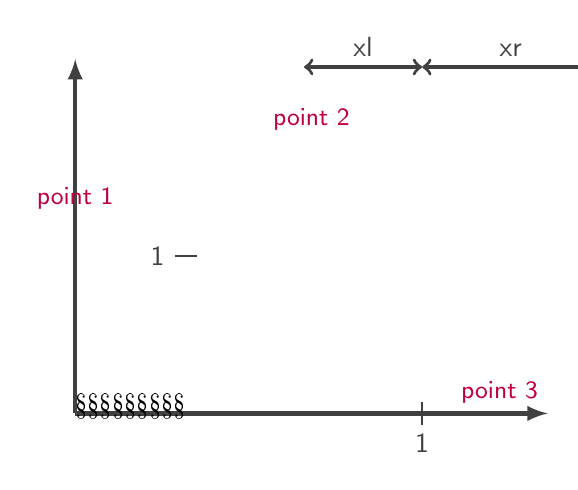
\begin{tikzpicture}[x=3cm,y=2cm,xmin=0,xmax=2,xgrilles=0.25,ymin=0,ymax=2.25,ygrilles=0.25]
	\tikzset{noeudexpl/.style={purple,font=\sffamily\small}}
	\tgrilles
	\draw[line width=1.5pt,->,darkgray,>=latex] (\xmin,0)--(\xmax,0) ;
	\draw[line width=1.5pt,->,darkgray,>=latex] (0,\ymin)--(0,\ymax) ;
	\draw (0,1.5) node[noeudexpl,below] {point 1} ;
	\draw (1,2) node[noeudexpl,below] {point 2} ;
	\draw (2,0) node[noeudexpl,above left] {point 3} ;
	%spline
	\SplineTikz[AffPoints,Coeffs=3§2,Couleur=red]{0/1.5/0§1/2/-0.333§2/0/-5}
	%tangente
	\TangenteTikz[xl=0,xr=0.5,Couleur=CouleurVertForet,Style=dashed]{0/1.5/0§1/2/-0.333§2/0/-5}
	\TangenteTikz[xl=0.5,xr=0.75,Couleur=orange,Style=dotted,Point=2]{0/1.5/0§1/2/-0.333§2/0/-5}
	\TangenteTikz[xl=0.33,xr=0,Couleur=blue,Style=densely dashed,Point=3]{0/1.5/0§1/2/-0.333§2/0/-5}
	%explications
	\draw[<->,very thick,darkgray] (0.5,2.2)--(1,2.2) node[midway,above,font=\sffamily] {xl} ;
	\draw[<->,very thick,darkgray] (1,2.2)--(1.75,2.2) node[midway,above,font=\sffamily] {xr};
	\draw[thick,darkgray] (1,4pt)--(1,-4pt) node[below,font=\sffamily] {1} ;
	\draw[thick,darkgray] (4pt,1)--(-4pt,1) node[left,font=\sffamily] {1} ;
\end{tikzpicture}
\end{center}
\end{PresCodeSortiePL}

\subsection{Exemple avec les deux outils, et \og personnalisation \fg}

\begin{PresCodeTexPL}{listing only}
\tikzset{%
	xmin/.store in=\xmin,xmin/.default=-5,xmin=-5,
	xmax/.store in=\xmax,xmax/.default=5,xmax=5,
	ymin/.store in=\ymin,ymin/.default=-5,ymin=-5,
	ymax/.store in=\ymax,ymax/.default=5,ymax=5,
	xgrille/.store in=\xgrille,xgrille/.default=1,xgrille=1,
	xgrilles/.store in=\xgrilles,xgrilles/.default=0.5,xgrilles=0.5,
	ygrille/.store in=\ygrille,ygrille/.default=1,ygrille=1,
	ygrilles/.store in=\ygrilles,ygrilles/.default=0.5,ygrilles=0.5,
	xunit/.store in=\xunit,unit/.default=1,xunit=1,
	yunit/.store in=\yunit,unit/.default=1,yunit=1
}

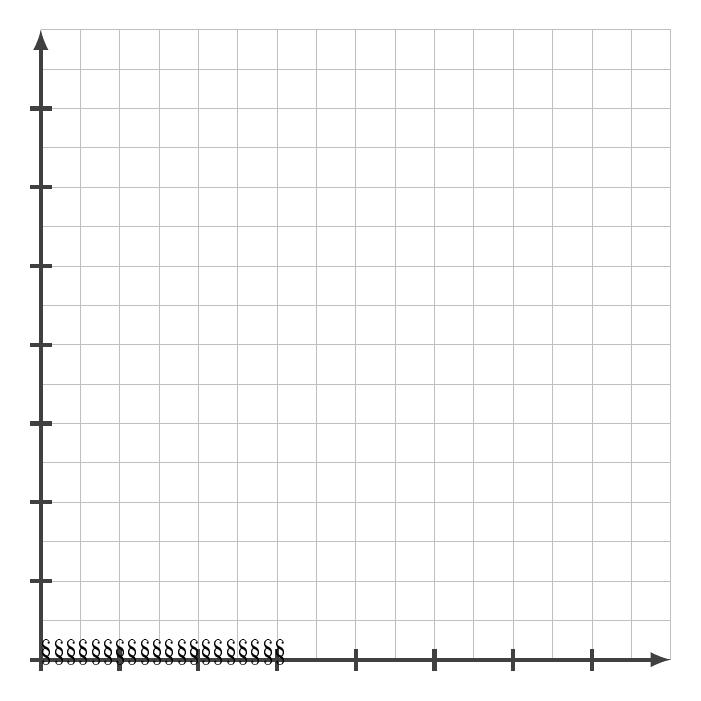
\begin{tikzpicture}[x=0.5cm,y=0.5cm,xmin=0,xmax=16,xgrilles=1,ymin=0,ymax=16,ygrilles=1]
	\draw[xstep=\xgrilles,ystep=\ygrilles,line width=0.3pt,lightgray] (\xmin,\ymin) grid (\xmax,\ymax) ;
	\draw[line width=1.5pt,->,darkgray,>=latex] (\xmin,0)--(\xmax,0) ;
	\draw[line width=1.5pt,->,darkgray,>=latex] (0,\ymin)--(0,\ymax) ;
	\foreach \x in {0,2,...,14} {\draw[darkgray,line width=1.5pt] (\x,4pt) -- (\x,-4pt) ;}
	\foreach \y in {0,2,...,14} {\draw[darkgray,line width=1.5pt] (4pt,\y) -- (-4pt,\y) ;}
	%la liste pour la courbe d'interpolation
	\def\liste{0/6/3§3/11/0§7/3/0§10/0/0§14/14/6}
	%les tangentes "stylisées"
	\TangenteTikz[xl=0,xr=1,Couleur=blue,Style=dashed]{\liste}
	\TangenteTikz[xl=2,xr=2,Couleur=purple,Style=dotted,Point=2]{\liste}
	\TangenteTikz[xl=2,xr=2,Couleur=orange,Style=<->,Point=3]{\liste}
	\TangenteTikz[xl=2,xr=0,Couleur=CouleurVertForet,Point=5]{\liste}
	%la courbe en elle-même
	\SplineTikz[AffPoints,Coeffs=3,Couleur=cyan,Style=densely dotted]{\liste}
\end{tikzpicture}
\end{PresCodeTexPL}

\begin{PresCodeSortiePL}{text only}
\begin{center}
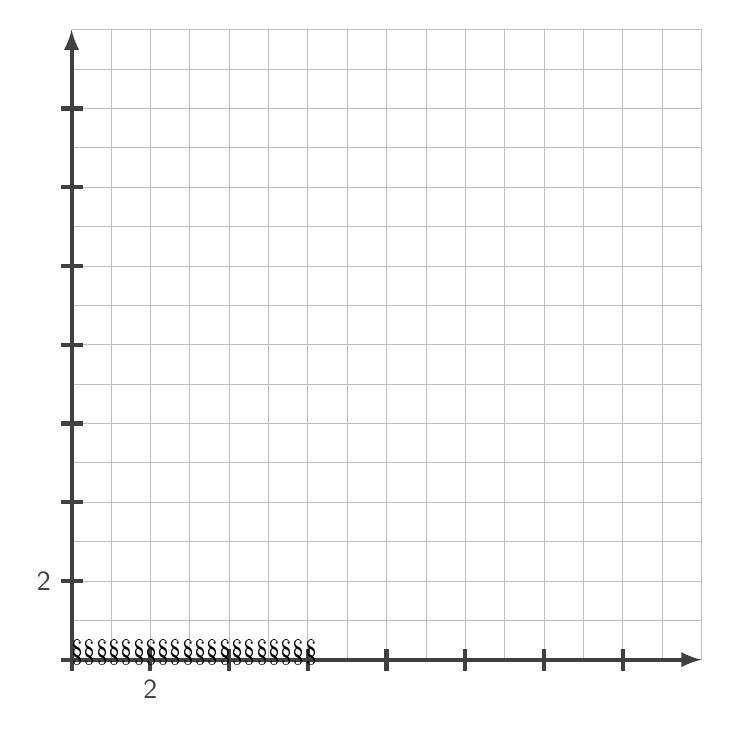
\begin{tikzpicture}[x=0.5cm,y=0.5cm,xmin=0,xmax=16,xgrilles=1,ymin=0,ymax=16,ygrilles=1]
	\draw[xstep=\xgrilles,ystep=\ygrilles,line width=0.3pt,lightgray] (\xmin,\ymin) grid (\xmax,\ymax) ;
	\draw[line width=1.5pt,->,darkgray,>=latex] (\xmin,0)--(\xmax,0) ;
	\draw[line width=1.5pt,->,darkgray,>=latex] (0,\ymin)--(0,\ymax) ;
	\foreach \x in {0,2,...,14} {\draw[darkgray,line width=1.5pt] (\x,4pt) -- (\x,-4pt) ;}
	\foreach \y in {0,2,...,14} {\draw[darkgray,line width=1.5pt] (4pt,\y) -- (-4pt,\y) ;}
	\draw[darkgray] (2,-4pt) node[below,font=\sffamily] {2} ;
	\draw[darkgray] (-4pt,2) node[left,font=\sffamily] {2} ;
	%la liste pour la courbe d'interpolation
	\def\liste{0/6/3§3/11/0§7/3/0§10/0/0§14/14/6}
	%les tangentes "stylisées"
	\TangenteTikz[xl=0,xr=1,Couleur=blue,Style=dashed]{\liste}
	\TangenteTikz[xl=2,xr=2,Couleur=purple,Style=dotted,Point=2]{\liste}
	\TangenteTikz[xl=2,xr=2,Couleur=orange,Style=<->,Point=3]{\liste}
	\TangenteTikz[xl=2,xr=0,Couleur=CouleurVertForet,Point=5]{\liste}
	%la courbe en elle-même
	\SplineTikz[AffPoints,Coeffs=3,Couleur=cyan,Style=densely dotted]{\liste}
\end{tikzpicture}
\end{center}
\end{PresCodeSortiePL}

\newpage

\section{Points de discontinuité}\label{discont}

\subsection{Idée}

\begin{tipblock}
\cmaj{2.7.7} L'idée est de présenter, en marge de la création de \textit{splines cubiques}, des points de discontinuité.

Pour des raisons \textit{internes} au code, cette possibilité n'est pas offerte (encore ?) directement dans la commande de création des splines.
\end{tipblock}

\begin{PresCodeTexPL}{listing only}
%dans un environnement tikz
\PtsDiscontinuite
\end{PresCodeTexPL}

\subsection{Commandes}

\begin{PresCodeTexPL}{listing only}
\begin{tikzpicture}[<options>]
	\PtsDiscontinuite{liste}[clés]
\end{tikzpicture}
\end{PresCodeTexPL}

\begin{cautionblock}
Le premier argument, \textit{optionnel} et entre \textsf{[...]}, contient les \Cle{Clés} suivantes :

\begin{itemize}
	\item la clé \Cle{Couleur} qui permet de définir la couleur du symbole ;\hfill{}défaut \Cle{red}
	\item la clé \Cle{Epaisseur} qui est relative à l'épaisseur du symbole ;\hfill{}défaut \Cle{1.25pt}
	\item la clé \Cle{Pos} pour choisir la position de la discontinuité (parmi \Cle{G/D}) ;\hfill{}défaut \Cle{D}
	\item la clé \Cle{Echelle} pour modifier l'échelle du symbole ;\hfill{}défaut \Cle{1}
	\item la clé \Cle{Type} pour choisir le type de symbole, parmi \Cle{par/cro/rond/demirond}.\hfill{}défaut \Cle{par}
\end{itemize}

Le second argument, obligatoire et entre \textsf{\{...\}} permet de préciser (comme pour les commandes des paragraphes précédents) la liste des points en lesquels le symbole de discontinuité sera positionné, sous la forme \verb|x1/y1/d1 § x2/y2/d2 § ...| avec les points \pverb|(xi;yi)| et \vverb|f'(xi)=di|.
\end{cautionblock}

\subsection{Exemples}

\begin{PresCodeTexPL}{listing only}
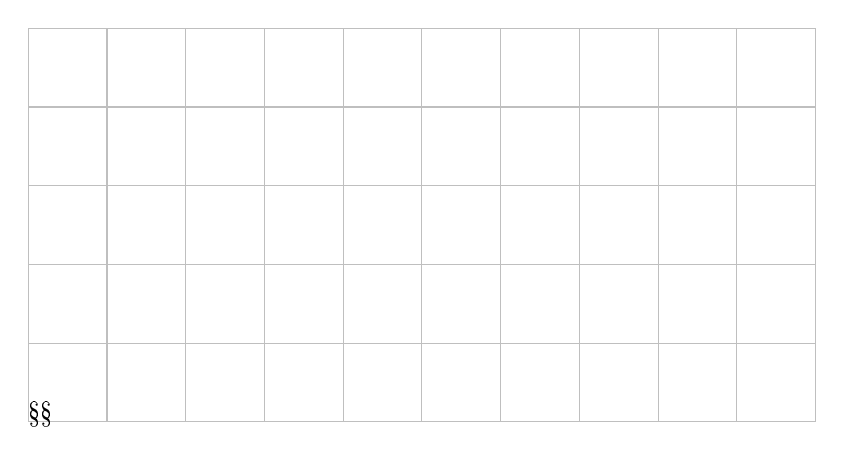
\begin{tikzpicture}
	\draw[lightgray] (0,0) grid (10,5) ;
	\SplineTikz{0/1/-1 § 4/4/0}
	\PtsDiscontinuite{4/4/0}
	\PtsDiscontinuite[Pos=G,Type=cro]{0/1/-1}
	\SplineTikz[Couleur=blue]{5/1/1.5 § 8/4/0.5}
	\PtsDiscontinuite[Couleur=blue,Type=rond]{8/4/0.5}
	\PtsDiscontinuite[Couleur=blue,Pos=G,Type=demirond,Echelle=2]{5/1/1.5}
\end{tikzpicture}
\end{PresCodeTexPL}

\begin{PresCodeTexPL}{text only}
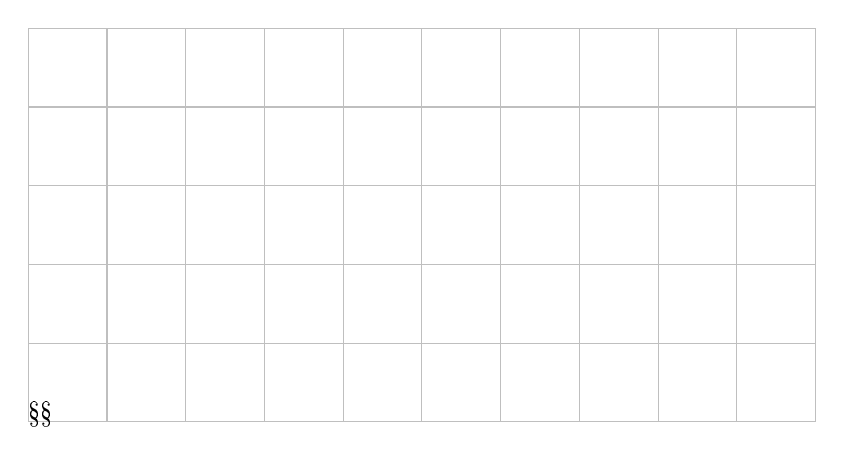
\begin{tikzpicture}
	\draw[lightgray] (0,0) grid (10,5) ;
	\SplineTikz{0/1/-1 § 4/4/0}
	\PtsDiscontinuite{4/4/0}
	\PtsDiscontinuite[Pos=G,Type=cro]{0/1/-1}
	\SplineTikz[Couleur=blue]{5/1/1.5 § 8/4/0.5}
	\PtsDiscontinuite[Couleur=blue,Type=rond]{8/4/0.5}
	\PtsDiscontinuite[Couleur=blue,Pos=G,Type=demirond,Echelle=2]{5/1/1.5}
\end{tikzpicture}
\end{PresCodeTexPL}

\newpage

\section{Petits schémas pour le signe de fonctions classiques}\label{aidesigne}

\subsection{Idée}

\begin{tipblock}
L'idée est d'obtenir une commande pour tracer (en \TikZ) un petit schéma pour \textit{visualiser} le signe d'une fonction affine ou d'un trinôme.

Le code est largement inspiré de celui du package \ctex{tnsana} même si la philosophie est un peu différente.

\smallskip

Comme pour les autres commandes \TikZ, l'idée est de laisser la possibilité à l'utilisateur de définir et créer son environnement \TikZ, et d'insérer la commande \ctex{MiniSchemaSignes} pour afficher le schéma.

\smallskip

\cmaj{2.1.9} Il est à noter que la version \textit{étoilée} rend la commande autonome, sans besoin de créer l'environnement \TikZ.
\end{tipblock}

\begin{PresCodePL}{}
\MiniSchemaSignes*
\end{PresCodePL}

\subsection{Commandes}

\begin{PresCodeTexPL}{listing only}
\begin{tikzpicture}[<options>]
	\MiniSchemaSignes[clés]
\end{tikzpicture}
\end{PresCodeTexPL}

\begin{PresCodeTexPL}{listing only}
{\tikz[options] \MiniSchemaSignes[clés]}
%ou
\MiniSchemaSignes*[clés]<options tikzpicture>
\end{PresCodeTexPL}

\begin{cautionblock}
\cmaj{2.1.9} La version \textit{étoilée} de la commande permet de basculer en mode \textit{autonome}, c'est-à-dire sans avoir besoin de créer son environnement \TikZ.

\smallskip

Le premier argument, \textit{optionnel} et entre \textsf{[...]}, contient les \Cle{Clés} suivantes :

\begin{itemize}
	\item la clé \Cle{Code} qui permet de définir le type d'expression (voir en-dessous) ;\hfill{}défaut \Cle{da+}
	\item la clé \Cle{Couleur} qui donne la couleur de la représentation ;\hfill{}défaut \Cle{red}
	\item la clé \Cle{Racines} qui définit la ou les racines ;\hfill{}défaut \Cle{2}
	\item la clé \Cle{Largeur} qui est la largeur du schéma ;\hfill{}défaut \Cle{2}
	\item la clé \Cle{Hauteur} qui est la hauteur du schéma ;\hfill{}défaut \Cle{1}
	\item un booléen \Cle{Cadre} qui affiche un cadre autour du schéma.\hfill{}défaut \Cle{true}
\end{itemize}

Le second argument, \textit{optionnel} et entre \textsf{<...>}, permet de spécifier (pour la commande \textit{étoilée}), des options à passer à l'environnement \ctex{tikzpicture}.
\end{cautionblock}

\begin{cautionblock}
Pour la clé \Cle{code}, il est construit par le type (\textsf{a} pour affine ou \textsf{p} comme parabole) puis les éléments caractéristiques (\textsf{a+} pour $a>0$, \textsf{d0} pour $\Delta=0$, etc) :

\begin{itemize}
	\item \Cle{Code=da+} := une droite croissante ;
	\item \Cle{Code=da-} := une droite décroissante ;
	\item \Cle{Code=pa+d+} := une parabole \textit{souriante} avec deux racines ;
	\item etc
\end{itemize}
\vspace*{-\baselineskip}\leavevmode
\end{cautionblock}

\pagebreak

\begin{PresCodeTexPL}{listing only}
\begin{center}
	\MiniSchemaSignes*[Code=da+,Racines=-4]
	~~~~
	\MiniSchemaSignes*[Code=da-,Racines={h},Couleur=blue,Largeur=3,Cadre=false]
\end{center}
%
\begin{center}
	\MiniSchemaSignes*[Code=pa+d+,Racines={1/2},Couleur=orange]
	~~~~
	\MiniSchemaSignes*[Code=pa+d-,Couleur=CouleurVertForet]
	~~~~
	\MiniSchemaSignes*[Code=pa+d0,Racines={5},Couleur=purple]
\end{center}
%
\begin{center}
	\MiniSchemaSignes*[Code=pa-d+,Racines={-3/0},Couleur=yellow]
	~~~~
	\MiniSchemaSignes*[Code=pa-d-,Couleur=cyan]
	~~~~
	\MiniSchemaSignes*[Code=pa-d0,Racines={-1},Couleur=magenta]
\end{center}
\end{PresCodeTexPL}

\begin{PresCodeSortiePL}{text only}
\begin{center}
	\MiniSchemaSignes*[Code=da+,Racines=-4]
	~~~~
	\MiniSchemaSignes*[Code=da-,Racines={h},Couleur=blue,Largeur=3,Cadre=false]
\end{center}
%
\begin{center}
	\MiniSchemaSignes*[Code=pa+d+,Racines={1/2},Couleur=orange]
	~~~~
	\MiniSchemaSignes*[Code=pa+d-,Couleur=CouleurVertForet]
	~~~~
	\MiniSchemaSignes*[Code=pa+d0,Racines={5},Couleur=purple]
\end{center}
%
\begin{center}
	\MiniSchemaSignes*[Code=pa-d+,Racines={-3/0},Couleur=yellow]
	~~~~
	\MiniSchemaSignes*[Code=pa-d-,Couleur=cyan]
	~~~~
	\MiniSchemaSignes*[Code=pa-d0,Racines={-1},Couleur=magenta]
\end{center}
\end{PresCodeSortiePL}

\begin{PresCodePL}{}
\begin{tikzpicture}
	\MiniSchemaSignes[Largeur=3.5,Hauteur=1.5,Code=da-,Racines=\tfrac{-b}{a},Couleur=pink]
\end{tikzpicture}

\MiniSchemaSignes*[Code=da-,Racines=\tfrac{-b}{a},Couleur=pink]<x=1.75cm,y=1.5cm>
\end{PresCodePL}

\pagebreak

\subsection{Intégration avec tkz-tab}

\begin{tipblock}
Ces schémas peuvent être de plus utilisés, via la commande \ctex{MiniSchemaSignesTkzTab} pour illustrer les signes obtenus dans un tableau de signes présentés grâce au package \ctex{tkz-tab}.

Pour des raisons internes, le fonctionnement de la commande \ctex{MiniSchemaSignesTkzTab} est légèrement différent et, pour des raisons que j'ignore, le code est légèrement différent en \textit{interne} (avec une \textit{déconnexion} des caractères \textsf{:} et \textsf{\textbackslash}) pour que la librairie \TikZ{} \ctex{calc} puisse fonctionner (mystère pour le moment\ldots)
\end{tipblock}

\begin{PresCodeTexPL}{listing only}
\begin{tikzpicture}
	%commandes tkztab
	\MiniSchemaSignesTkzTab[options]{numligne}[echelle][décalage horizontal]
\end{tikzpicture}
\end{PresCodeTexPL}

\begin{cautionblock}
Les \Cle{Clés} pour le premier argument \textit{optionnel} sont les mêmes que pour la version \textit{initiale} de la commande précédente.

En ce qui concerne les autres arguments :

\begin{itemize}
	\item le deuxième argument, \textit{obligatoire}, est le numéro de la ligne à côté de laquelle placer le schéma ;
	\item le troisième argument, \textit{optionnel} et valant \Cle{0.85} par défaut, est l'échelle à appliquer sur l'ensemble du schéma (à ajuster en fonction de la hauteur de la ligne) ;
	\item le quatrième argument, \textit{optionnel} et valant \Cle{1.5} par défait, est lié à l'écart horizontal entre le bord de la ligne du tableau et le schéma.
\end{itemize}

À noter que si l'un des arguments optionnels (le n°3 et/ou le n°4) sont utilisés, il vaut mieux préciser les 2 !
\end{cautionblock}

\begin{PresCodeTexPL}{listing only}
\begin{center}
\begin{tikzpicture}
	\tkzTabInit[]{$x$/1,$-2x+5$/1,$2x+4$/1,$p(x)$/1}{$-\infty$,$-2$,${2,5}$,$+\infty$}
	\tkzTabLine{,+,t,+,z,-,}
	\tkzTabLine{,-,z,+,t,+,}
	\tkzTabLine{,-,z,+,z,-,}
	\MiniSchemaSignesTkzTab[Code=da-,Racines={\tfrac{5}{2}},Couleur=blue]{1}
	\MiniSchemaSignesTkzTab[Code=da+,Racines={-2},Couleur=purple]{2}
	\MiniSchemaSignesTkzTab[Code=pa-d+,Racines={-2/{\tfrac{5}{2}}},Couleur=orange]%
		{3}[0.85][2]
\end{tikzpicture}
\end{center}
\end{PresCodeTexPL}

\begin{PresCodeSortiePL}{text only}
\begin{center}
\begin{tikzpicture}
	\tkzTabInit[]{$x$/1,$-2x+5$/1,$2x+4$/1,$p(x)$/1}{$-\infty$,$-2$,${2,5}$,$+\infty$}
	\tkzTabLine{,+,t,+,z,-,}
	\tkzTabLine{,-,z,+,t,+,}
	\tkzTabLine{,-,z,+,z,-,}
	\MiniSchemaSignesTkzTab[Code=da-,Racines={\tfrac{5}{2}},Couleur=blue]{1}
	\MiniSchemaSignesTkzTab[Code=da+,Racines={-2},Couleur=purple]{2}
	\MiniSchemaSignesTkzTab[Code=pa-d+,Racines={-2/{\tfrac{5}{2}}},Couleur=orange]{3}[0.85][2]
\end{tikzpicture}
\end{center}
\end{PresCodeSortiePL}

\newpage

\section{Ligne de convexité en lien avec tkz-tab}\label{tkzconvex}

\subsection{Idée}

\begin{tipblock}
\cmaj{3.02c} L'idée est d'obtenir une commande pour rajouter une ligne de \textit{convexité} dans un tableau créé par \ctex{tkz-tab}.

Cette commande est donc à utiliser dans un environnement correctement défini par les macros de \ctex{tkz-tab} car elle utilise les \textit{nœuds} créés.
\end{tipblock}

\begin{PresCodeTexPL}{listing only}
\begin{tikzpicture}
	%commandes tkztab
	\tkzTabLineConvex(*){num ligne}{liste 'cases'}
\end{tikzpicture}
\end{PresCodeTexPL}

\subsection{Commande}

\begin{cautionblock}
La version \textit{étoilée} permet de forcer l'affichage des attributs en mode \textit{texte}.

Le premier argument, \textit{obligatoire} et entre \Cle{\{...\}}, est le numéro de la ligne sur laquelle on souhaite afficher les attributs de convexité.

Le second argument, \textit{obligatoire} et entre \Cle{\{...\}}, donne -- en langage \texttt{tkz-tab}, le contenu de la ligne de convexité, avec les même \textit{règles} pour pour les commandes de \ctex{tkz-tab}, avec en plus :

\begin{itemize}
	\item \Cle{i*} := point d'inflexion (avec \textit{texte}) ;
	\item \Cle{i} := point d'inflexion (sans texte) ;
	\item \Cle{ccv} := concave (schéma, ou texte en mode \textit{étoilé}) ;
	\item \Cle{cvx} := convexe (schéma, ou texte en mode \textit{étoilé}).
\end{itemize}
\vspace*{-\baselineskip}\leavevmode
\end{cautionblock}

\begin{PresCodePL}{}
\begin{tikzpicture}
	\tkzTabInit[lgt=3,espcl=4]{$x$/1,$f''(x)$/1,Convexité\\de $f$/2}{$0$,$1$,$3$,$5$}
	\tkzTabLine{,+,z,-,z,+,}
	\tkzTabLineConvex{2}{,cvx,i*,ccv,i*,cvx,}
\end{tikzpicture}
\end{PresCodePL}

\begin{PresCodePL}{}
\begin{tikzpicture}
	\tkzTabInit[lgt=3,espcl=4]{$x$/1,$f''(x)$/1,Convexité\\de $f$/2}{$0$,$1$,$3$,$5$}
	\tkzTabLine{,+,z,-,z,+,}
	\tkzTabLineConvex*{2}{,cvx,i,ccv,i,cvx,}
\end{tikzpicture}
\end{PresCodePL}

\begin{PresCodePL}{}
\begin{tikzpicture}
	\tkzTabInit[lgt=3,espcl=4]{$x$/1,$f''(x)$/1,Convexité\\de $f$/2}{$0$,$1$,$3$,$5$}
	\tkzTabLine{,+,z,-,d,+,}
	\tkzTabLineConvex*{2}{,cvx,t,ccv,d,cvx,}
\end{tikzpicture}
\end{PresCodePL}

\newpage

\section{Suites récurrentes et \og toile \fg}\label{recurr}

\subsection{Idée}

\begin{tipblock}
L'idée est d'obtenir une commande pour tracer (en \TikZ) la \og toile \fg{} permettant d'obtenir -- graphiquement -- les termes d'une suite récurrente définie par une relation $u_{n+1}=f(u_n)$.

\smallskip

Comme pour les autres commandes \TikZ, l'idée est de laisser l'utilisateur définir et créer son environnement \TikZ, et d'insérer la commande \ctex{ToileRecurrence} pour afficher la \og toile \fg.
\end{tipblock}

\subsection{Commandes}

\begin{PresCodeTexPL}{listing only}
...
\begin{tikzpicture}[options]
...
\ToileRecurrence[clés][options du tracé][options supplémentaires des termes]
...
\end{tikzpicture}
\end{PresCodeTexPL}

\begin{cautionblock}
Plusieurs \Cle{arguments} (optionnels) sont disponibles :

\begin{itemize}
\item le premier argument optionnel définit les \Cle{Clés} de la commande :
\begin{itemize}
	\item la clé \Cle{Fct} qui définit la fonction $f$ ;\hfill{}défaut \Cle{vide}
	\item la clé \Cle{Nom} qui est le \textit{nom} de la suite ;\hfill{}défaut \Cle{u}
	\item la clé \Cle{No} qui est l'indice initial ;\hfill{}défaut \Cle{0}
	\item la clé \Cle{Uno} qui est la valeur du terme initial ;\hfill{}défaut \Cle{vide}
	\item la clé \Cle{Nb} qui est le nombre de termes à construire ;\hfill{}défaut \Cle{5}
	\item la clé \Cle{PosLabel} qui est le placement des labels par rapport à l'axe $(Ox)$ ;\hfill{}défaut \Cle{below}
	\item la clé \Cle{DecalLabel} qui correspond au décalage des labels par rapport aux abscisses ;
	
	\hfill{}défaut \Cle{6pt}
	\item la clé \Cle{TailleLabel} qui correspond à la taille des labels ;\hfill{}défaut \Cle{small}
	\item un booléen \Cle{AffTermes} qui permet d'afficher les termes de la suite sur l'axe $(Ox)$.
	
	\hfill{}défaut \Cle{true}
\end{itemize}
\item le deuxième argument optionnel concerne les \Cle{options} du tracé de l'\textit{escalier} en \textit{langage \TikZ} ;

\hfill{}défaut \Cle{thick,color=magenta} ;
\item le troisième argument optionnel concerne les \Cle{options} du tracé des termes en \textit{langage \TikZ}.

\hfill{}défaut \Cle{dotted}.
\end{itemize}
\vspace*{-\baselineskip}\leavevmode
\end{cautionblock}

\begin{noteblock}
Il est à noter que le \textsf{code} n'est pas autonome, et doit être intégré dans un environnement \ctex{tikzpicture}.

\smallskip

L'utilisateur est donc libre de définir ses styles pour l'affichage des éléments de son graphique, et il est libre également de rajouter des éléments en plus du tracé de la \textit{toile} !

\smallskip

La macro ne permet -- pour le moment -- ni de tracer la bissectrice, ni de tracer la courbe$\ldots$

En effet, il y aurait trop d'options pour ces deux éléments, et l'idée est quand même de conserver une commande \textit{simple} ! Donc l'utilisateur se chargera de tracer et de personnaliser sa courbe et sa bissectrice !
\end{noteblock}

\subsection{Exemples}

\begin{noteblock}
On va tracer la \textit{toile} des 4 premiers termes de la suite récurrente : \[\begin{dcases} u_1 = 1 \\ u_{n+1} = \sqrt{5u_n}+1 \text{ pour tout entier } n \geqslant 1\end{dcases}\]
\end{noteblock}

\begin{PresCodePL}{tikz lower}
%code tikz
\def\x{1.5cm}\def\y{1.5cm}
\def\xmin{0}\def\xmax{10}\def\xgrille{1}\def\xgrilles{0.5}
\def\ymin{0}\def\ymax{8}\def\ygrille{1}\def\ygrilles{0.5}
%axes et grilles
\draw[xstep=\xgrilles,ystep=\ygrilles,line width=0.6pt,lightgray!50] (\xmin,\ymin) grid (\xmax,\ymax);
\draw[line width=1.5pt,->,darkgray,>=latex] (\xmin,0)--(\xmax,0) ;
\draw[line width=1.5pt,->,darkgray,>=latex] (0,\ymin)--(0,\ymax) ;
\foreach \x in {0,1,...,9} {\draw[darkgray,line width=1.5pt] (\x,4pt) -- (\x,-4pt) ;}
\foreach \y in {0,1,...,7} {\draw[darkgray,line width=1.5pt] (4pt,\y) -- (-4pt,\y) ;}
%fonction définie et réutilisable
\def\f{sqrt(5*\x)+1}
%toile
\ToileRecurrence[Fct={\f},No=1,Uno=1,Nb=4,DecalLabel=4pt]
%éléments supplémentaires
\draw[very thick,blue,domain=0:8,samples=250] plot (\x,{\f}) ;
\draw[very thick,CouleurVertForet,domain=0:8,samples=2] plot (\x,\x) ;
\end{PresCodePL}

\begin{noteblock}
Peut-être que -- ultérieurement -- des options \textit{booléennes} seront disponibles pour un tracé \textit{générique} de la courbe et de la bissectrice, mais pour le moment la \textsf{macro} ne fait \textit{que} l'escalier.
\end{noteblock}

\subsection{Influence des paramètres}

\begin{PresCodeTexPL}{listing only}
\begin{center}
\begin{tikzpicture}[x=4cm,y=3cm]
%axes + grilles + graduations
...
%fonction
\def\f{-0.25*\x*\x+\x}
%tracés
\begin{scope}
	\clip (0,0) rectangle (2.5,1.25) ;
	\draw[line width=1.25pt,blue,domain=0:2.5,samples=200] plot (\x,{\f}) ;
\end{scope}
\ToileRecurrence[Fct={\f},No=0,Uno=2,Nb=5,PosLabel=above right,DecalLabel=0pt]
\end{tikzpicture}
\end{center}
\end{PresCodeTexPL}

\begin{PresCodeSortiePL}{text only}
\begin{center}
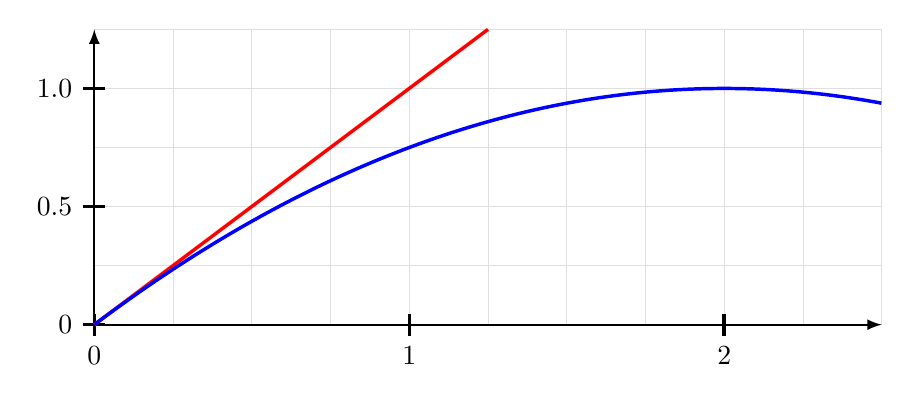
\begin{tikzpicture}[x=4cm,y=3cm]
	\draw[xstep=0.25,ystep=0.25,line width=0.3pt,lightgray!50] (0,0) grid (2.5,1.25);
	\draw[thick,->,>=latex] (0,0)--(2.5,0) ;
	\draw[thick,->,>=latex] (0,0)--(0,1.25) ;
	\foreach \x in {0,1,2}
	\draw[line width=1.25pt] (\x,4pt) -- (\x,-4pt) node[below] {\num{\x}} ;
	\foreach \y in {0,0.5,1.0}
	\draw[line width=1.25pt] (4pt,\y) -- (-4pt,\y) node[left] {\num{\y}} ;
	\draw[line width=1.25pt,red](0,0) -- (1.25,1.25) ;
	%fonction
	\def\f{-0.25*\x*\x+\x}
	%tracés
	\begin{scope}
				\clip (0,0) rectangle (2.5,1.25) ;
				\draw[line width=1.25pt,blue,domain=0:2.5,samples=200] plot (\x,{\f}) ;
			\end{scope}
	\ToileRecurrence[Fct={\f},No=0,Uno=2,Nb=5,PosLabel=above right,DecalLabel=0pt]
\end{tikzpicture}
\end{center}
\end{PresCodeSortiePL}

\begin{PresCodeTexPL}{listing only}
\begin{center}
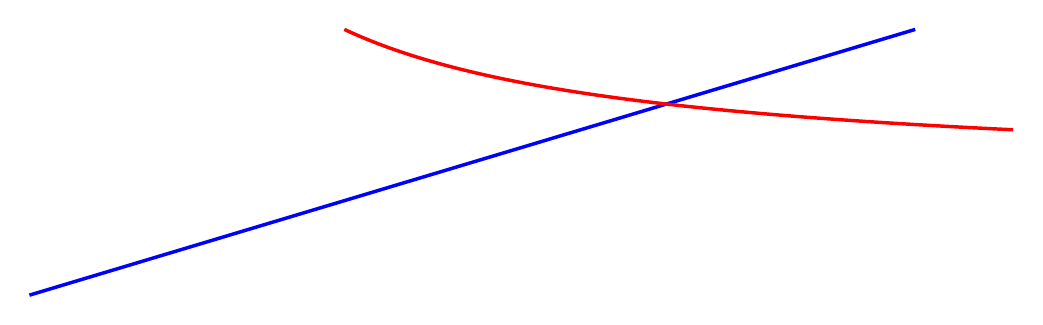
\begin{tikzpicture}[x=5cm,y=1.5cm]
	...
	\def\f{1+1/\x}
	\ToileRecurrence%
		[Fct={\f},No=0,Uno=1,Nb=7,PosLabel=above right,DecalLabel=0pt,AffTermes=false]%
		[line width=1.25pt,CouleurVertForet,densely dashed][]
	\draw[line width=1.25pt,blue,domain=0:2.25,samples=2] plot(\x,{\x});
	\draw[line width=1.25pt,red,domain=0.8:2.5,samples=250] plot(\x,{\f});
\end{tikzpicture}
\end{center}
\end{PresCodeTexPL}

\begin{PresCodeSortiePL}{text only}
\begin{center}
	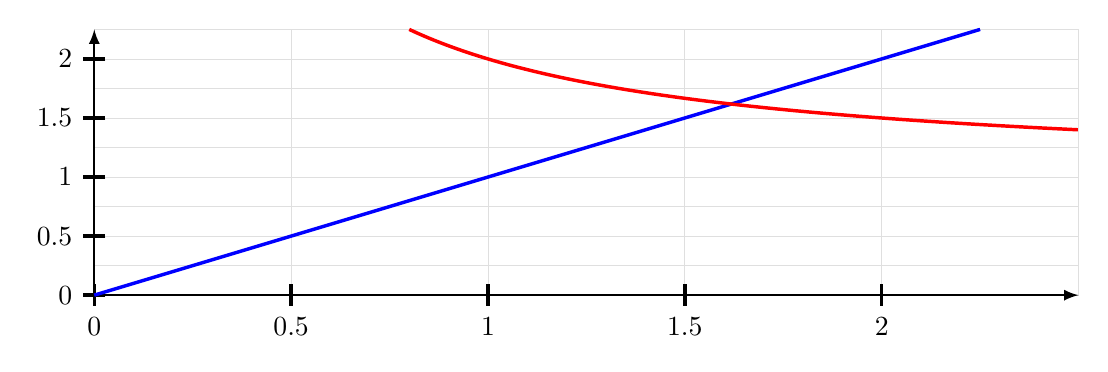
\begin{tikzpicture}[x=5cm,y=1.5cm]
			%axes et grille
			\draw[xstep=0.5,ystep=0.25,line width=0.3pt,lightgray!50] (0,0) grid (2.5,2.25);
			\draw[thick,->,>=latex] (0,0)--(2.5,0) ;
			\draw[thick,->,>=latex] (0,0)--(0,2.25) ;
			\foreach \x in {0,0.5,...,2}
				\draw[line width=1.25pt] (\x,4pt) -- (\x,-4pt) node[below] {\num{\x}};
			\foreach \y in {0,0.5,...,2}
				\draw[line width=1.25pt] (4pt,\y) -- (-4pt,\y) node[left] {\num{\y}};
			%fonction
			\def\f{1+1/\x}
			%tracés
			\ToileRecurrence%
				[Fct={\f},No=0,Uno=1,Nb=7,PosLabel=above right,DecalLabel=0pt,AffTermes=false]%
				[line width=1.25pt,CouleurVertForet,densely dashed][]
			\draw[line width=1.25pt,blue,domain=0:2.25,samples=2] plot(\x,{\x});
			\draw[line width=1.25pt,red,domain=0.8:2.5,samples=250] plot(\x,{\f});
		\end{tikzpicture}
\end{center}
\end{PresCodeSortiePL}

\newpage

\section{Méthodes graphiques et intégrales}\label{integrtikz}

\subsection{Idées}

\begin{tipblock}
\cmaj{2.6.1} L'idée est de proposer plusieurs méthodes graphiques pour illustrer graphiquement une intégrale, via :
\begin{itemize}
	\item une méthode des rectangles (Gauche, Droite ou Milieu) ;
	\item la méthode des trapèzes.
\end{itemize}
La commande n'est pas autonome, elle est de ce fait à être placée dans un environnement \ctex{tikzpicture}.

\smallskip

\cmaj{3.04a} Il est également possible d'afficher le domaine défini par une intégrale, sans méthode numérique particulière.
\end{tipblock}

\begin{PresCodeTexPL}{listing only}
%commande pour déclarer une fonction réutilisable, en langage TikZ
\DeclareFonctionTikz[nom]{expr}

%commande pour déclarer une fonction réutilisable, en langage xint
\DeclareFonctionTikzXint[nom]{expr}
\end{PresCodeTexPL}

\begin{PresCodeTexPL}{listing only}
%environnement tikz
\IntegraleApprocheeTikz[clés]{nom_fonction}{a}{b}
\end{PresCodeTexPL}

\begin{PresCodeTexPL}{listing only}
%environnement tikz
\IntegraleTikz[clés]<options tikz>{fct1}[fct2]{a}{b}     %version tikz
\IntegraleTikzXint[clés]<options tikz>{fct1}[fct2]{a}{b} %version xint
\end{PresCodeTexPL}

\subsection{Intégrales simples}

\begin{cautionblock}
Plusieurs \Cle{Clés} sont disponibles pour la commande \textit{simple} :

\begin{itemize}
	\item la clé \Cle{Epaisseur} pour l'épaisseur des \og figures \fg{} ; \hfill~défaut : \Cle{1pt}
	\item la clé \Cle{Couleurs} pour les couleurs (\Cle{Bordure/intérieur}) \fg{} ; \hfill~défaut : \Cle{gray/teal}
	\item la clé \Cle{Style}, pour remplir les \og figures \fg{} (\Cle{remplissage/hachures}) ; \hfill~défaut : \Cle{remplissage}
	\item la clé \Cle{Opacite} pour l'opacité du remplissage des \og figures \fg{} ;
	
	\hfill~défaut : \Cle{0.5}
	\item la clé \Cle{Hachures} pour le style des hachures (\ctex{pattern})
	
	\hfill~défaut : \Cle{north west lines}
	\item la clé \Cle{Type}, parmi \Cle{dessous/entre} ;\hfill~défaut : \Cle{dessous}
	\item la clé \Cle{Jonction}, pour le type de jonction des portions ;\hfill~défaut : \Cle{bevel}
	\item la clé \Cle{Pas} (si \Cle{Xint}).\hfill~défaut : \Cle{0.1}
\end{itemize}

\smallskip

Le deuxième argument, optionnel et entre \ctex{<...>}, correspond à des options spécifiques à passer au tracé.

\smallskip

Concernant les arguments suivants, correspondant aux éléments du tracé :

\begin{itemize}
	\item le premier est la fonction (en langage \TikZ\ ou \ctex{xint}) ;
	\item le deuxième est la fonction n°2 (si \Cle{Type=entre} en langage \TikZ\ ou \ctex{xint}) ;
	\item le troisième est la borne inférieure ;
	\item le dernière est la borne supérieure.
\end{itemize}

Les commandes graphiques de \ctex{Proflycee} peuvent être utilisées pour configure la fenêtre !
\end{cautionblock}

\begin{PresCodePL}{}
\begin{tikzpicture}%
	[x=0.66cm,y=0.033cm,xmin=0,xmax=21,xgrille=2,xgrilles=1,ymin=0,ymax=160,ygrille=20,ygrilles=10]
	\DeclareFonctionTikz{80*\x*exp(-0.2*\x)}
	\GrilleTikz
	\IntegraleTikz{f(\x)}{3}{17}
	\AxesTikz\AxexyTikz{0,2,...,20}{0,20,...,160}
	\CourbeTikz[very thick,samples=500,blue]{f(\x)}{1:20}
\end{tikzpicture}
\end{PresCodePL}

\begin{PresCodePL}{}
\begin{tikzpicture}%
	[x=0.66cm,y=0.033cm,xmin=0,xmax=21,xgrille=2,xgrilles=1,ymin=0,ymax=160,ygrille=20,ygrilles=10]
	\DeclareFonctionTikzXint[K]{80*x*exp(-0.2*x)}
	\DeclareFonctionTikzXint[L]{10*x}
	\GrilleTikz
	\IntegraleTikzXint[Type=entre,Style=hachures,Hachures=bricks]{K(x)}[L(x)]{3}{10}
	\AxesTikz\AxexyTikz{0,2,...,20}{0,20,...,160}
	\CourbeTikzXint[very thick,blue]{K(x)}{1..[0.1]..20}
	\CourbeTikzXint[very thick,red]{L(x)}{1..[10]..20}
\end{tikzpicture}
\end{PresCodePL}

\subsection{Clés et arguments pour les méthodes approchées}

\begin{cautionblock}
Plusieurs \Cle{Clés} sont disponibles pour la commande \textit{approchée} :

\begin{itemize}
	\item la clé \Cle{Epaisseur} pour l'épaisseur des \og figures \fg{} ; \hfill~défaut : \Cle{semithick}
	\item la clé \Cle{Couleur} pour la couleur des \og figures \fg{} ; \hfill~défaut : \Cle{red}
	\item le booléen \Cle{Remplir}, pour remplir les \og figures \fg{} ; \hfill~défaut : \Cle{true}
	\item la clé \Cle{Opacite} pour l'opacité du remplissage des \og figures \fg{} ;
	
	\hfill~défaut : \Cle{0.25}
	\item la clé \Cle{CouleurRemplissage} pour la couleur de remplissage des \og figures \fg{} ;
	
	\hfill~défaut : \Cle{Couleur!25}
	\item la clé \Cle{Methode}, parmi \Cle{RectanglesGauche / RectanglesDroite / RectanglesMilieu / Trapezes} pour spécifier la méthode utilisée ;
	
	\hfill~défaut : \Cle{RectanglesGauche}
	\item la clé \Cle{NbSubDiv} précise le nombre de \og figures \fg{}. \hfill~défaut : \Cle{10}
\end{itemize}

\smallskip

Concernant les arguments obligatoires :

\begin{itemize}
	\item le premier est la fonction , déclarée au préalable ;
	\item les deux autres arguments sont les bornes de l'intégrale.
\end{itemize}

Les commandes graphiques de \ctex{Proflycee} peuvent être utilisées pour configure la fenêtre !
\end{cautionblock}

\begin{PresCodePL}{}
\begin{tikzpicture}%
	[x=0.66cm,y=0.033cm,xmin=0,xmax=21,xgrille=2,xgrilles=1,ymin=0,ymax=160,ygrille=20,ygrilles=10]
	\DeclareFonctionTikz{80*\x*exp(-0.2*\x)}
	\FenetreSimpleTikz{0,2,...,20}{0,20,...,160}
	\CourbeTikz[very thick,samples=500,blue]{f(\x)}{1:20}
	\IntegraleApprocheeTikz{f}{1}{20}
	\draw[red] (10,160) node[below right]
		{$\displaystyle%
		\IntegraleApprochee[Methode=RectanglesGauche,AffFormule,Expr={80x\,\text{e}^{-0,2x}}]%
		{80*x*exp(-0.2*x)}{1}{20}$} ;
\end{tikzpicture}
\end{PresCodePL}

\begin{PresCodePL}{}
\begin{tikzpicture}%
	[x=0.66cm,y=0.033cm,xmin=0,xmax=21,xgrille=2,xgrilles=1,ymin=0,ymax=160,ygrille=20,ygrilles=10]
	\DeclareFonctionTikz{80*\x*exp(-0.2*\x)}
	\FenetreSimpleTikz{0,2,...,20}{0,20,...,160}
	\CourbeTikz[very thick,samples=500,blue]{f(\x)}{1:20}
	\IntegraleApprocheeTikz[NbSubDiv=76]{f}{1}{20}
	\draw[red] (10,160) node[below right]
		{$\displaystyle\IntegraleApprochee%
		[NbSubDiv=76,Methode=RectanglesGauche,AffFormule,Expr={80x\,\text{e}^{-0,2x}}]%
		{80*x*exp(-0.2*x)}{1}{20}$} ;
\end{tikzpicture}
\end{PresCodePL}

\pagebreak

\subsection{Exemples}

\begin{PresCodePL}{}
\begin{tikzpicture}%
	[x=0.66cm,y=0.033cm,xmin=0,xmax=21,xgrille=2,xgrilles=1,ymin=0,ymax=160,ygrille=20,ygrilles=10]
	\DeclareFonctionTikz{80*\x*exp(-0.2*\x)}
	\FenetreSimpleTikz{0,2,...,20}{0,20,...,160}
	\CourbeTikz[very thick,samples=500,blue]{f(\x)}{1:20}
	\IntegraleApprocheeTikz[Methode=RectanglesDroite,Couleur=green]{f}{1}{20}
	\draw[green] (10,160) node[below right]
	{$\displaystyle\IntegraleApprochee%
		[Methode=RectanglesDroite,AffFormule,Expr={80x\,\text{e}^{-0,2x}}]%
		{80*x*exp(-0.2*x)}{1}{20}$} ;
\end{tikzpicture}
\end{PresCodePL}

\begin{PresCodePL}{}
\begin{tikzpicture}%
	[x=0.66cm,y=0.033cm,xmin=0,xmax=21,xgrille=2,xgrilles=1,ymin=0,ymax=160,ygrille=20,ygrilles=10]
	\DeclareFonctionTikz{80*\x*exp(-0.2*\x)}
	\FenetreSimpleTikz{0,2,...,20}{0,20,...,160}
	\CourbeTikz[very thick,samples=500,blue]{f(\x)}{1:20}
	\IntegraleApprocheeTikz[Methode=RectanglesMilieu,Couleur=purple]{f}{1}{20}
	\draw[purple] (10,160) node[below right]
	{$\displaystyle\IntegraleApprochee%
		[Methode=RectanglesMilieu,AffFormule,Expr={80x\,\text{e}^{-0,2x}}]%
		{80*x*exp(-0.2*x)}{1}{20}$} ;
\end{tikzpicture}
\end{PresCodePL}

\begin{PresCodePL}{}
\begin{tikzpicture}%
	[x=0.66cm,y=0.033cm,xmin=0,xmax=21,xgrille=2,xgrilles=1,ymin=0,ymax=160,ygrille=20,ygrilles=10]
	\DeclareFonctionTikz{80*\x*exp(-0.2*\x)}
	\FenetreSimpleTikz{0,2,...,20}{0,20,...,160}
	\CourbeTikz[very thick,samples=500,blue]{f(\x)}{1:20}
	\IntegraleApprocheeTikz[Methode=Trapezes,Couleur=orange]{f}{1}{20}
	\draw[orange] (10,160) node[below right]
	{$\displaystyle\IntegraleApprochee%
		[Methode=Trapezes,AffFormule,Expr={80x\,\text{e}^{-0,2x}}]%
		{80*x*exp(-0.2*x)}{1}{20}$} ;
\end{tikzpicture}
\end{PresCodePL}